%%%%%%%%%%%%%%%%%%%% author.tex %%%%%%%%%%%%%%%%%%%%%%%%%%%%%%%%%%%
%
% sample root file for your "contribution" to a proceedings volume
%
% Use this file as a template for your own input.
%
%%%%%%%%%%%%%%%% Springer %%%%%%%%%%%%%%%%%%%%%%%%%%%%%%%%%%


\documentclass{svproc}
%
% RECOMMENDED %%%%%%%%%%%%%%%%%%%%%%%%%%%%%%%%%%%%%%%%%%%%%%%%%%%
%

% to typeset URLs, URIs, and DOIs
\usepackage{url}
\def\UrlFont{\rmfamily}

\usepackage{listings}
\usepackage{color}

\definecolor{dkgreen}{rgb}{0,0.6,0}
\definecolor{gray}{rgb}{0.5,0.5,0.5}
\definecolor{mauve}{rgb}{0.58,0,0.82}

\lstset{frame=tb,
  language=Java,
  aboveskip=3mm,
  belowskip=3mm,
  showstringspaces=false,
  columns=flexible,
  basicstyle={\small\ttfamily},
  numbers=none,
  numberstyle=\tiny\color{gray},
  keywordstyle=\color{blue},
  commentstyle=\color{dkgreen},
  stringstyle=\color{mauve},
  breaklines=true,
  breakatwhitespace=true,
  tabsize=3
}



\usepackage{graphicx}

\usepackage{booktabs}

\usepackage[table,xcdraw]{xcolor}




\begin{document}
\mainmatter              % start of a contribution
%
\title{Deep Learning with Keras}
%
\titlerunning{Deep Learning with Keras}  % abbreviated title (for running head)
%                                     also used for the TOC unless
%                                     \toctitle is used
%
\author{Mohd Zamri Murah}
%
%\authorrunning{Ivar Ekeland et al.} % abbreviated author list (for running head)
%
%%%% list of authors for the TOC (use if author list has to be modified)
%\tocauthor{Ivar Ekeland, Roger Temam, Jeffrey Dean, David Grove,
%Craig Chambers, Kim B. Bruce, and Elisa Bertino}
%
\institute{Center of Artificial Intelligence Technology\\ 
Fakulti Teknologi Sains Maklumat\\
Universiti Kebangsaan Malaysia\\
\email{zamri@ukm.edu.my}}

\maketitle              % typeset the title of the contribution

\begin{abstract}
This technical report is a preliminary study of deep learning using Keras. We experiments deep six learning models on MNIST datasets. From the experiments, we observe the following conclusions. First, deep learning is very flexible and we can create many type of models and layers. Second, the experiments require GPU-based machine to shorten the time for each experiments. Third, the models are domain specified, not a general purpose model.

\keywords{deep learning, Keras, Python}
\end{abstract}
%
\section{Introduction}
%

Deep learning refers to artificial neural networks that are composed of many layers. 
It's a growing trend in ML due to some favorable results in applications where the target function is very complex and the datasets are large\cite{hinton2012improving}. An algorithm is deep if the input is passed through several non-linearities before being output. Most modern learning algorithms (including decision trees and SVMs and naive bayes) are "shallow". Deep learning is motivated by intuition, theoretical arguments from circuit theory, empirical results, and current knowledge of neuroscience.

Deep Learning is about learning multiple levels of representation and abstraction that help to make sense of data such as images, sound, and text.

\section{Literature Review}

In machine learning and cognitive science, artificial neural networks (ANNs) are a family of models inspired by biological neural networks (the central nervous systems of animals, in particular the brain) and are used to estimate or approximate functions that can depend on a large number of inputs and are generally unknown. Artificial neural networks are generally presented as systems of interconnected "neurons" which exchange messages between each other. The connections have numeric weights that can be tuned based on experience, making neural nets adaptive to inputs and capable of learning.

\begin{figure}
% https://en.wikibooks.org/wiki/LaTeX/Importing_Graphics
% Use the relevant command to insert your figure file.
% For example, with the graphicx package use
\centering{\fbox{\includegraphics[scale=.35]{ann.png}}}
% figure caption is below the figure
\caption{Artificial Neural Network}
\label{fig:1}       % Give a unique label
\end{figure}



Deep learning is called "deep" because of the structure of ANNs. Earlier 40 years back, neural networks were only 2 layers deep as it was not computationally feasible to build larger networks. Now it is common to have neural networks with 10+ layers and even 100+ layer ANNs are being tried upon.


\begin{figure}
% https://en.wikibooks.org/wiki/LaTeX/Importing_Graphics
% Use the relevant command to insert your figure file.
% For example, with the graphicx package use
 \centering{\fbox{\includegraphics[scale=0.6]{dl_layers.png}}}
% figure caption is below the figure
\caption{Layers of neurons}
\label{fig:1}       % Give a unique label
\end{figure}

DL is essentially stack layers of neurons on top of each other. The lowest layer takes the raw data like images, text, sound, etc. and then each neurons stores some information about the data they encounter. Each neuron in the layer sends information up to the next layers of neurons which learn a more abstract version of the data below it. So the higher you go up, the more abstract features you learn.  DL systems are ANN that are constructed with multiple layers (sometimes called Multi-level Perceptrons).



\section{Keras}

Keras\cite{chollet2015keras} is a high-level neural networks library, written in Python\cite{van2007python} and capable of running on top of either TensorFlow\cite{abadi2015tensorflow} or Theano\cite{bergstra2011theano}.


%\begin{lstlisting}
%// Hello.java
%import javax.swing.JApplet;
%import java.awt.Graphics;
%
%public class Hello extends JApplet {
%    public void paintComponent(Graphics g) {
%        g.drawString("Hello, world!", 65, 95);
%    }    
%}
%\end{lstlisting}

\lstinputlisting[language=Python,caption=Python code for multi-leyer perceptron]{mnist_mlp.py}
%\begin{lstlisting}[language=Python, caption=Python example]
%
%\end{lstlisting}


A deep learning model based on multi-layer perceptron\cite{cirecsan2012deep} on the MNIST dataset is given in figure~\ref{fig:1}.
A simple convnet\cite{sermanet2012convolutional} on the MNIST dataset is given in figure~\ref{fig:2}. 

A Net2Net deep learning is given in figure~\ref{fig:3} and figure~\ref{fig:4}.  Net2Net is a group of methods to transfer knowledge from a teacher neural net to a student net,so that the student net can be trained faster than from scratch. This enable 'lifelong learning system' by gradually adjusting model complexity
    to data availability,and reusing transferable knowledge.


\begin{figure}
% https://en.wikibooks.org/wiki/LaTeX/Importing_Graphics
% Use the relevant command to insert your figure file.
% For example, with the graphicx package use
 \centering{\fbox{\includegraphics[scale=0.4,angle=90]{model_mlp.png}}}
% figure caption is below the figure
\caption{Deep learning architecture for multi-layers perceptrons}
\label{fig:1}       % Give a unique label
\end{figure}



\begin{figure}
% https://en.wikibooks.org/wiki/LaTeX/Importing_Graphics
% Use the relevant command to insert your figure file.
% For example, with the graphicx package use
 \centering{\fbox{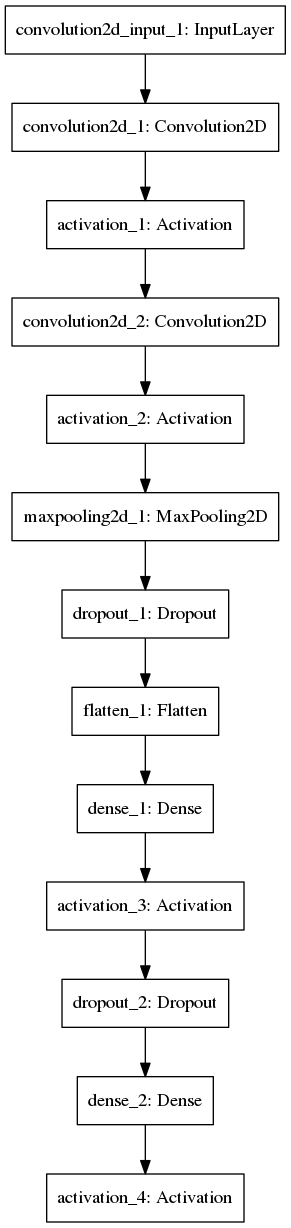
\includegraphics[scale=0.35,angle=90]{model_cnn.png}}}
% figure caption is below the figure
\caption{Deep learning architecture for convolution network}
\label{fig:2}       % Give a unique label
\end{figure}



\begin{figure}
% https://en.wikibooks.org/wiki/LaTeX/Importing_Graphics
% Use the relevant command to insert your figure file.
% For example, with the graphicx package use
 \centering{\fbox{\includegraphics[scale=0.4,angle=90]{model_net2net_teacher.png}}}
% figure caption is below the figure
\caption{Deep learning architecture for teacher in Net2Net network}
\label{fig:3}       % Give a unique label
\end{figure}

\begin{figure}
% https://en.wikibooks.org/wiki/LaTeX/Importing_Graphics
% Use the relevant command to insert your figure file.
% For example, with the graphicx package use
 \centering{\fbox{\includegraphics[scale=0.4,angle=90]{model_net2net_student.png}}}
% figure caption is below the figure
\caption{Deep learning architecture for student in Net2Net network}
\label{fig:4}       % Give a unique label
\end{figure}

\section{Results}

The experiments is done on MNIST dataset\cite{lecun-mnisthandwrittendigit-2010}. The MNIST dataset is a dataset of handwritten digits, comprising 60 000 training examples and 10 000 test examples. The dataset can be downloaded from http://yann.lecun.com/exdb/mnist/. 

All experiments are done on a Linux Ubuntu 16.04 with Intel i5 and 8GB RAM. No GPU is used. These experiments indicates that to do deep learning models, we need GPU-supported machines. Without GPU, the time requires to implement the models is long.


% Please add the following required packages to your document preamble:
% \usepackage{booktabs}
% \usepackage[table,xcdraw]{xcolor}
% If you use beamer only pass "xcolor=table" option, i.e. \documentclass[xcolor=table]{beamer}
% http://www.tablesgenerator.com/
% Please add the following required packages to your document preamble:
% \usepackage{booktabs}
% \usepackage[table,xcdraw]{xcolor}
% If you use beamer only pass "xcolor=table" option, i.e. \documentclass[xcolor=table]{beamer}
\begin{table}[]
\centering
\begin{tabular}{@{}lllll@{}}
\toprule
\textbf{method} & \textbf{epoch} & \textbf{accuracy} & \textbf{params} & \textbf{time} \\ \midrule
\textit{\begin{tabular}[c]{@{}l@{}}CNN (convolution \\ neural network)\end{tabular}} &  12 & 0.99 & 600810  &  35m\\
\rowcolor[HTML]{ECF4FF} 
\textit{\begin{tabular}[c]{@{}l@{}}MLP (multilayer \\ perceptron)\end{tabular}} &  20 &  0.9828 &  669706&  5m \\
\textit{Net2Net} &  3 & 0.9958 &  238986 & 132m \\
\rowcolor[HTML]{ECF4FF} 
\textit{\begin{tabular}[c]{@{}l@{}}IRNN (Initialize \\ Recurrent Networks)\end{tabular}} &  200 &  0.93 &  11210 & 30h  \\
\textit{\begin{tabular}[c]{@{}l@{}}Siamese multi-layer \\ perceptron\end{tabular}} &  20 & 0.995 &  133504 &  4m \\
\rowcolor[HTML]{ECF4FF} 
\textit{Hierarchical RNN} &  5 &  0.9858 &  199434 & 150m  \\ \bottomrule
\end{tabular}
\caption{Experimental results using six types of deep learning networks on MNIST dataset.}
\label{my-label}
\end{table}
%
% ---- Bibliography ----

\pagebreak

\bibliography{keras}
%\bibliographystyle{splncs_srt}
\bibliographystyle{spmpsci}

\end{document}
